In the section the approach followed to build the CCN will be described.
\subsection{Overall setup}
A deep CNN will be trained to give a probability distribution over the phonemes labels given the acoustic input. The acoustic input will be converted into a sequence of fixed size frames windows, that is converted into spectrograms. The deep CNN will then generate probability distributions over the possible phone labels for each spectrogram. The sequence of the probability distributions will then be used to compute the emission probabilities of the HMM states on a Viterbi decoder that can generate the expected phones sequence.\\\\
In this work, the CCN network ability to predict the correct phone label given an input spectrogram was tested, and no Viterbi decoder was used.
\subsection{Feature representation}
As in \cite{graves2014towards} we have chosen to use the spectrograms as inputs to the CCN. The acoustic input are split into smaller frames chunks which are then converted into fixed size spectrogram images. Section \ref{sec:spect} detail the spectrograms generation process for this phone recognition task.

\subsection{Network Architecture}
As suggested in \cite{sainath2013deep}, a CNN network with both convolutional layers and fully connected layers will be used. Convolutional layers will be used at the first (bottom) layers of the network, while fully connected layers will be used at the last (top) layers of the network. The convolutional layers will sometimes be followed with a pooling layer. Having the convolutional layers at the bottom of the network helps with the spectral variation, and the fully connected layer are used to discriminate between the different phonemes using the convoluted-pooled input from the convolution and pooling layers.
\\
Our architecture follows after the famous AlexNet\cite{NIPS2012_4824}, a very successful network used in Computer Vision literature to do object recognition on more than 1,000 classes. Figure~\ref{fig:net} shows the architecture of the best performing network according to our experiments. As we will see in Section~\ref{sec:experiments}, we have tried slightly modified versions of this architecture for different experiment.

\begin{figure}
\centering
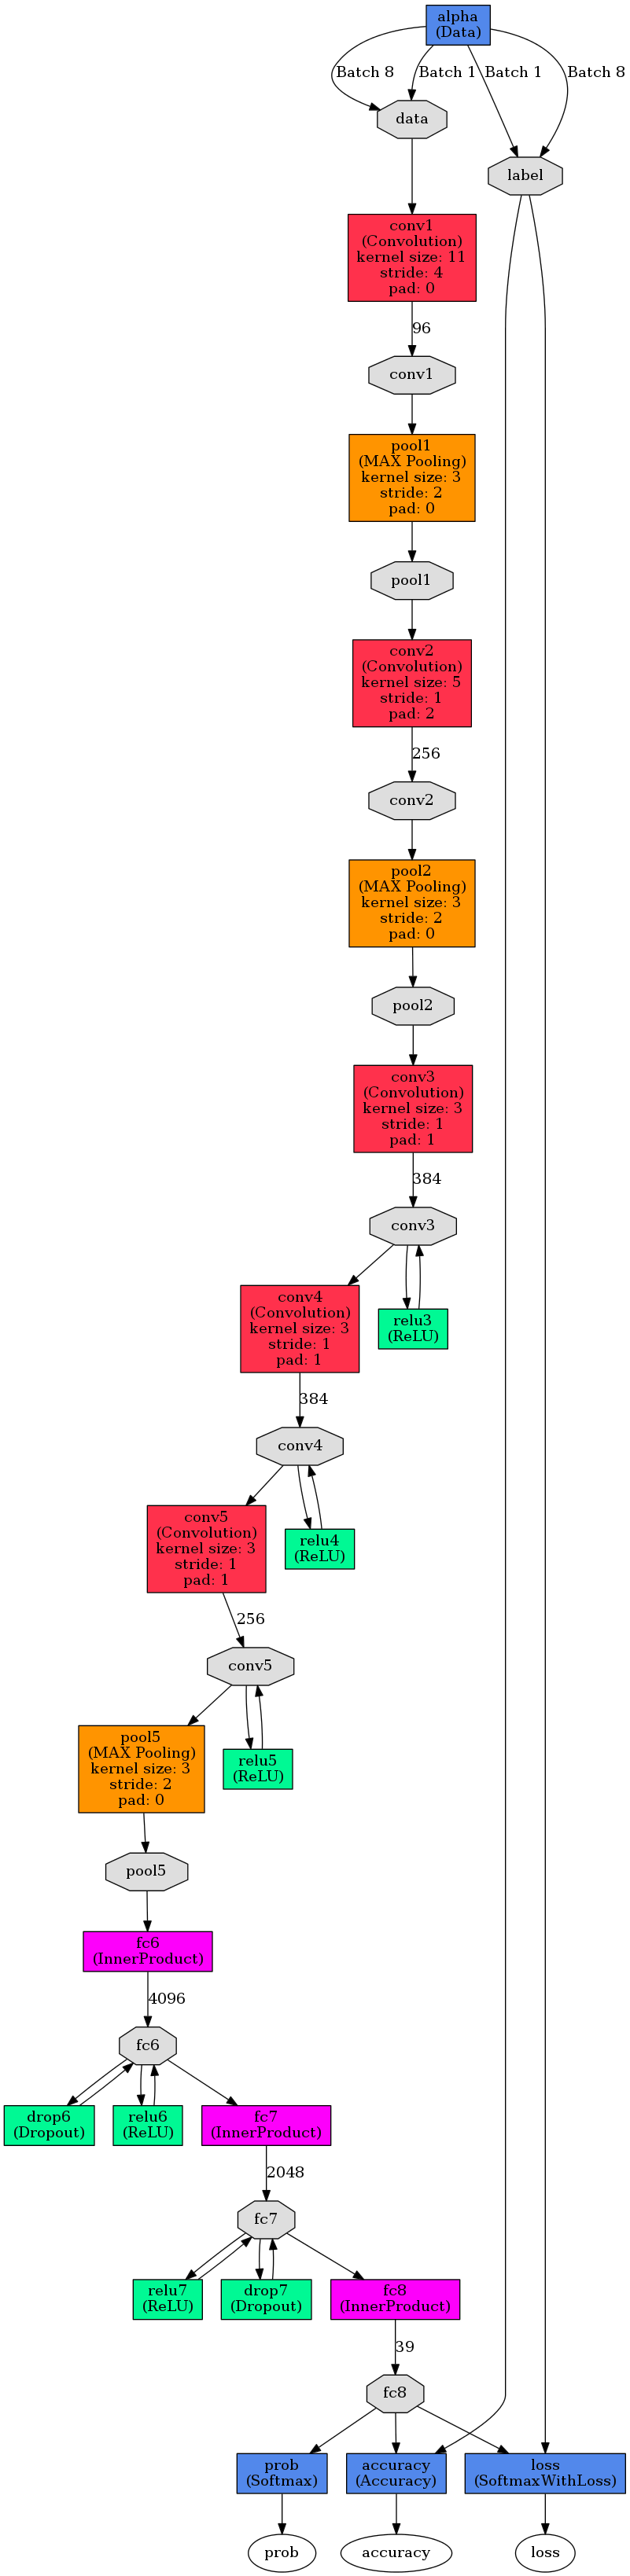
\includegraphics[scale=0.2]{figs/alexnet}
\caption{\label{fig:net}Best performing network architecture, it follows after AlexNet.}
\end{figure}
\subsection{Evaluation}
A number of CNN with different number of layers will be trained. The performance of these networks will be compared using the classification error rate. Due to the limitation of the computing resources, a relatively small networks will be trained, also the network will be trained to classify over a subset of the phonemes.